\chapter{Provas de Cross Country}\label{cha:tasks}

O XCSoar fornece um sistema completo de gerenciamento de provas, no qual as provas podem ser editadas priorizando o vôo e quando se voa cross-country casual, podem ser modificadas durante o vôo.  Os waypoints podem ser avançados automaticamente ou manualmente.  Muitos cálculos do XCSoar são relativos aos pilões ou ao waypoint final.  A menos que uma prova real seja definida, o XCSoar irá criar uma função ‘casa’ com muitas das funções da prova, referindo-se à localização da decolagem.  Este capítulo também descreve o uso do registrador IGC com o XCSoar.

Existem três modos de provas disponíveis:

\begin{description}
\item[Prova ordenada] esta é a prova tradicional de cross-country, na qual consiste em um ponto de início, zero ou mais waypoints e um waypoint final.  Os pontos da prova têm que ser voados em ordem.
\item[Prova 'Ir Para'] voa-se para um único destino.
\item[Abortar prova] fornece opção para se voar ao próximo ponto pousável.
\end{description}

Observe que nos modos Ir para e Abortar Prova, a prova ordenada é retida e pode ser retomada posteriormente, preservando todas as estatísticas sobre as realizações na prova.

\subsection*{‘Ir para’ automático}

Se não houver nenhuma prova ordenada definida, haverá uma prova de ‘ir para’ definida automaticamente na decolagem, definindo a decolagem como ponto de destino ou o próximo aeródromo se estiver perto do ponto da decolagem.

Se houver ou não prova definida, o ponto de decolagem é sempre gerado e aparecerá na lista de waypoints para referências futuras.

Após a prova ordenada ter sido definida pela primeira vez, a função “ir para’ decolagem é ignorada.  Para retomar uma prova simples, use ‘Ir para’.


\section{Provas “Ir Para”}

As provas ‘Ir Para’ podem ser definidas selecionando um waypoint no mapa, pela lista de waypoints ou outro mecanismo, como por exemplo uma caixa de diálogo, e selecione  \bmenuw{Vá Para}. No modo de prova, selecione
\bmenug{Nav 2} e então \blink\bmenug{Prova} {Retomar} e a prova será retomada (se houver alguma).
 

\section{Editando provas}

Você pode editar provas de várias maneiras. Alguns métodos são mais úteis para editar antes do vôo e outros permitem que a prova seja modificada em vôo.  As provas podem ser salvas em arquivos e carregadas posteriormente e podem ser transferidas entre qualquer plataforma que rode o XCSoar.

\tip Também é possível salvar uma prova padrão e tê-la carregada automaticamente no início do XCSoar.  Uma utilização para isto é que você pode fazer uma prova com somente um waypoint e ajustá-lo para ‘casa’ – significa que o XCSoar será programado para voar de volta a esse ponto, que pode ser útil para se voar local.

As principais maneiras de configurar uma prova são:
\begin{itemize}
\item Usando a caixa de diálogo de edição de prova.
\item Selecionando o waypoint no mapa e adicionando-o à prova através da janela de diálogo de waypoint.
\item Carregando a prova a partir de um arquivo.
\end{itemize}

%Selecting the Task menu item will produce the Task dialogue box.  The
%list box on the left displays all of the turn points loaded into the
%system. Highlight the desired entries and using the "-$>$" and "$<$-"
%buttons assemble the desired task in the Task list box. As each turn
%point is added to the task a continuous display of the calculated task
%length is shown.  Tasks can be saved for recalling later using the
%"Save" button and recalled using the "Load" button.  Once the desired
%task is complete select "OK".
%
%{\it DIAGRAM SHOWING TASK DIALOG EDITING, WITH LABELED ARROWS POINTING
%TO THE USER INTERFACE ELEMENTS?}

Carregar uma prova através de um arquivo talvez seja útil em competição ou cross-country quando voado em grupo, já que um só piloto pode distribuir o arquivo aos outros, economizando tempo de todos para editar a prova.  Se não houver prova ativa no início, o XCSoar criará automaticamente uma prova contendo o waypoint ‘casa’.

O XCSoar salva a prova atual quando é desligado e carrega-a assim que ligado, permitindo que se possa desligar o XCSoar até voar novamente.

Os pontos da prova são preservados mesmo que o waypoint seja alterado.  Isto significa que, se você tem uma prova e altera um arquivo de waypoint e carregar a prova novamente, novos waypoints serão gerados para os pontos que estão faltando no novo arquivo de waypoint.



\section{Informação do Waypoint }
%Several ways of selecting a waypoint are available:
%\begin{itemize}
%\item Touch its name or the waypoint symbol on the map screen if it is visible.
%\item If the waypoint is in the active task, highlight the waypoint {\InfoBox}, 
%  then use the up/down arrow keys to select the desired waypoint, and press the
%enter key.
%\item From the Task dialogue, find and highlight the waypoint in
% the waypoint list, then press the 'Details' button.
%\end{itemize}
%The display will now show the waypoint details dialogue.

A janela de diálogo do waypoint descreve os detalhes deste ponto e tem suas funções de navegação como Ir, Inserir, Anexar à prova ou ajustar este waypoint à nova posição ‘casa’.  Pode ser acessado das seguintes formas:

\gesturespec{rd}ou menu \bmenug{Nav 1/2}\blink\bmenug{Prova},
\todonum{descr. tabular "Pilões"}
selecione um waypoint, clique novamente no waypoint para mostrar a janela de diálogo deste ponto, e então clique em\bmenuw{Detalhes}.

\gesturespec{dl}ou menu \bmenug{Nav 1/2}\blink\bmenug{Alternativos}
para mostrar os detalhes dos pontos pousáveis perto da aeronave.

\gesturespec{dr}ou menu \bmenug{Nav 1/2}\blink\bmenug{Lista Waypoint}
, selecione e\bmenuw{Selec} para selecionar o waypoint e mostrar os detalhes.

\gesturespec{urdl}or menu \bmenug{Display 1/2}\blink\bmenug{Pan On} para colocar o mapa em modo panorâmico, arrastando até o ponto desejado do waypoint, tocando seu nome ou seu símbolo

\bmenug{Info 1/3}\blink\bmenug{Oque aqui?}
para mostrar a lista de itens abaixo da mira da tela, ou seu dedo no mapa.


Os detalhes do waypoint contém duas páginas principais (acessadas através dos botões 
\bmenuw{$>$} e \bmenuw{$<$}). do waypoint, podem ser mostrados em páginas extras.

\subsection*{Detalhes do Waypoint}
\label{sec:waypointdetails}
Esta página contém texto descritivo da localização do waypoint, frequência de rádio e informações da pista (se houver esta informação no arquivo de waypoints), elevação, hora do nascer e pôr do sol, direção, distancia ao waypoint e altitude necessária para atingir o waypoint. Também há um botão 
\bmenuw{IR} para iniciar imediatamente a navegação a este waypoint.  Este botão cancela a prova atual.

\begin{center}
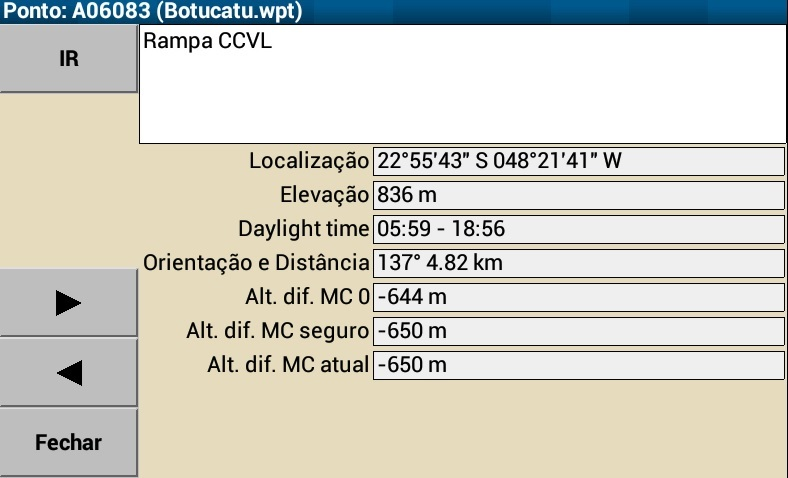
\includegraphics[angle=0,width=0.8\linewidth,keepaspectratio='true']{figures/dialog-waypointdetails0.png}
\end{center}

Como citado acima, a janela de diálogo do waypoint também mostra três formas de diferença de altitude (altitude adicional necessária para alcançar o waypoint a uma altura segura) para o waypoint correspondente:
\begin{description}
\item[Alt diff MC 0] Diferença de altitude com MC ajustado em 0.
\item[Alt diff MC safety] Diferença de altitude no ajuste de segurança/aborto de MacCready (veja seção  \ref{sec:safety-factor})
\item[Alt diff MC current] Diferença de altitude com o ajuste atual de MacCready.
\end{description}

Através da janela principal de waypoint, você pode acessar a segunda página usando os botões 
\bmenuw{$>$} e \bmenuw{$<$} no canto inferior esquerdo da tela.  
\subsection*{Menu de ações da prova}  
Esta página contém uma coluna de botões que permite várias ações:
\begin{description}
\item[\bmenuw{Substituir na prova}] substitui o waypoint ativo na prova pelo waypoint selecionado.
\item[\bmenuw{Inserir na prova}] insere o waypoint selecionado antes do waypoint ativo na prova.
\item[\bmenuw{Anexar à prova}] adiciona o waypoint selecionado ao final da prova.
\item[\bmenuw{Remover da prova}] remove o waypoint selecionado da prova.  Esta opção só estará visíviel se o waypoint selecionado está incluso na prova.
\item[\bmenuw{Selec como nova Casa}] ajusta o waypoint como ‘casa’.
\item[\bmenuw{Deslocar para waypoint}] alterna para o modo panorâmico e arrasta para o waypoint.
\end{description}

É uma boa idéia ajustar seu waypoint ‘casa’ na janela de diálogo de waypoints.  Isto faz o XCSoar iniciar sempre neste ponto, mesmo quando o XCSoar ainda não obteve sua posição de GPS.  Se não for fixada nenhuma posição 'casa', o XCSoar irá centrar no meio do mapa.

\subsection*{Informação do Aeródromo}
Esta página pode conter texto relevante sobre o aeródromo, incluindo pistas, frequências de rádio, padrões de tráfego e contatos.
\begin{center}
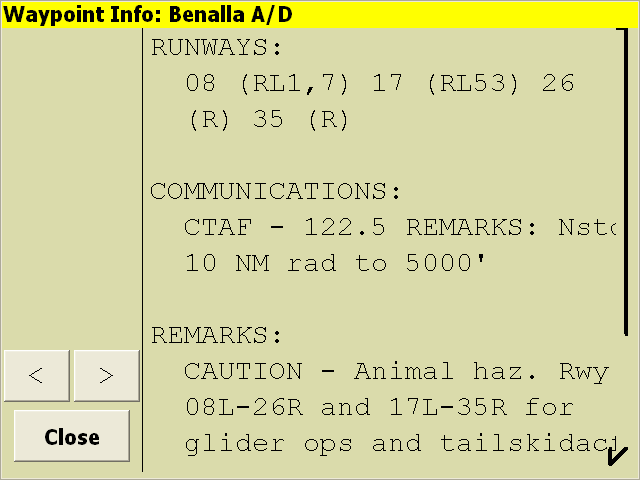
\includegraphics[angle=0,width=0.8\linewidth,keepaspectratio='true']{figures/dialog-waypointdetails1.png}
\end{center}

\subsection*{Imagem dos detalhes do Waypoint}
Esta página mostra uma imagem de satélite do waypoint.

\begin{center}
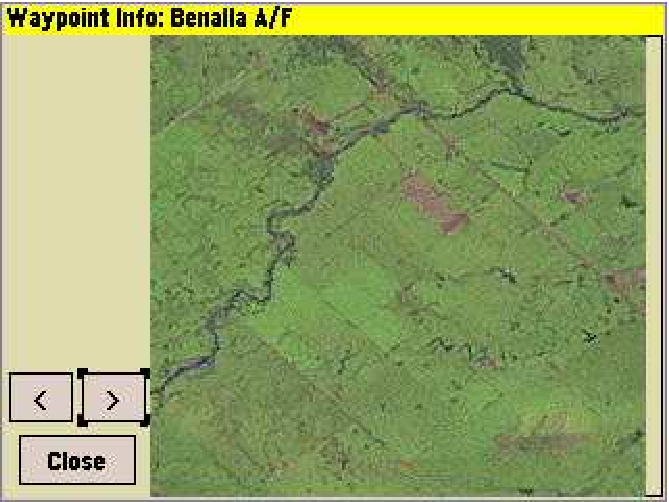
\includegraphics[angle=0,width=0.8\linewidth,keepaspectratio='true']{figures/dialog-waypointdetails2.pdf}
\end{center}
Como ajustar as informações de detalhes do waypoint estão na seção \ref{sec:airfield-details}

\section{A janela de seleção de Waypoint}\label{sec:waypoint-selector-dialog}

A janela de seleção do waypoint permite que se selecione facilmente de um grande banco de dados.  \gesturespec{dr}

Acionando a seleção ativa uma tela com um conjunto de filtros do lado 
\menulabelr{\bmenug{Nav 1/2}\blink\bmenug{Lista Waypoint}}
esquerdo da tela e uma lista de waypoints do lado direito da tela, coincidindo todas as condições dos filtros.  Há vários filtros disponíveis, que podem ser usados em conjunto, individuais ou sem filtro.
\begin{description}
\item[Nome] seleciona os waypoints começando com o caractere digitado.
\item[Distância] filtra os waypoints mais próximos do que a distância digitada.
\item[Direção] filtra os waypoints que não estão especificados na direção da aeronave.  A direção especial “HDG(0°)” filtra waypoints com até 30° de deslocamento para ambos os lados do sentido da aeronave.  Isto permite que o piloto aponte a aeronave a um grupo de waypoints e rapidamente possa achá-los.
\item[Tipo] filtra waypoints que não são do tipo especificado (pousáveis, aeroportos ou pilões) ou que aparecem em arquivos específicos.
\end{description}
Quando filtrados por nome e tipo, a listra é mostrada em ordem alfabética.  Quando filtrado por distância ou direção, a lista é ordenada por distância.  

\begin{center}
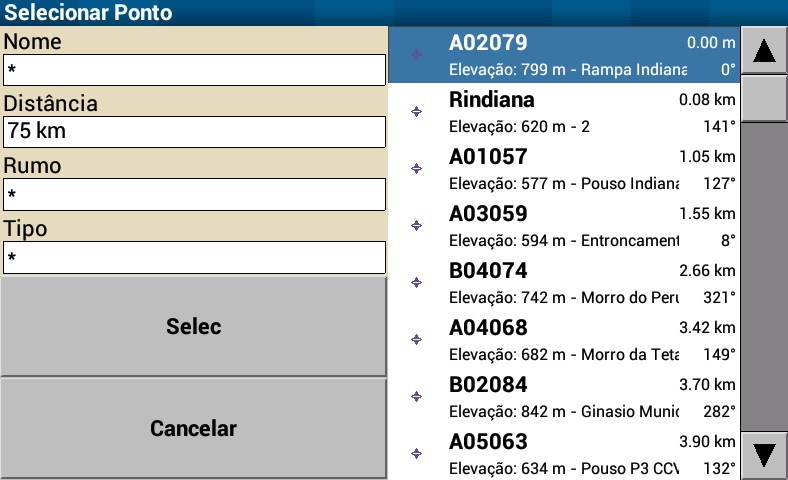
\includegraphics[angle=0,width=0.8\linewidth,keepaspectratio='true']{figures/dialog-waypointselect.png}
\end{center}

A lista pode ser rolada se houver mais de uma tela cheia de waypoints.  Para rolar a lista, simplesmente arraste com o dedo ou mova para baixo (ou para cima) a lista com o cursor. 

Selecionar um item irá resultar em um comportamento diferente, dependendo de qual função abriu o seletor de waypoints.  No uso normal, mostrará os detalhes do waypoint.

\section{Gerenciador de Tarefas}\label{sec:task-manager-dialog}
\begin{it}  O gerenciador de tarefas foi redesenhado se comparado com as versões anteriores do XCSoar.\end{it}
\gesturespec{rd}

O gerenciador de tarefas é usado para editar, visualizar, carregar, salvar em arquivo e declarar as provas de cross-country.
\menulabelr{\bmenug{Nav 1/2}\blink\bmenug{Prova}}

A primeira página é uma calculadora.  Mostra vários cálculos relativos à prova ativa, como descrito em detalhes abaixo:  Há botões para acionar os diálogos \bmenuw{Pilões}, \bmenuw{Gerenciar}, 
e \bmenuw{Regras}, bem como o botão \bmenuw{Fechar} .

\subsection*{Janela de Calculadora de Prova}\label{sec:task-calc-dial}
A janela calculadora de prova permite que o piloto veja o efeito de suas várias mudanças da prova no desempenho final.
\menulabelr{\bmenuw{Calculadora}}

Em vôo, a Calculadora de Prova também pode ser acessada da página de Análise.  Com as páginas Prova, Subida e Velocidade da Prova, aparece um botão chamado  \bmenuw{Calculadora} que vai diretamente à esta janela.
 



\begin{center}
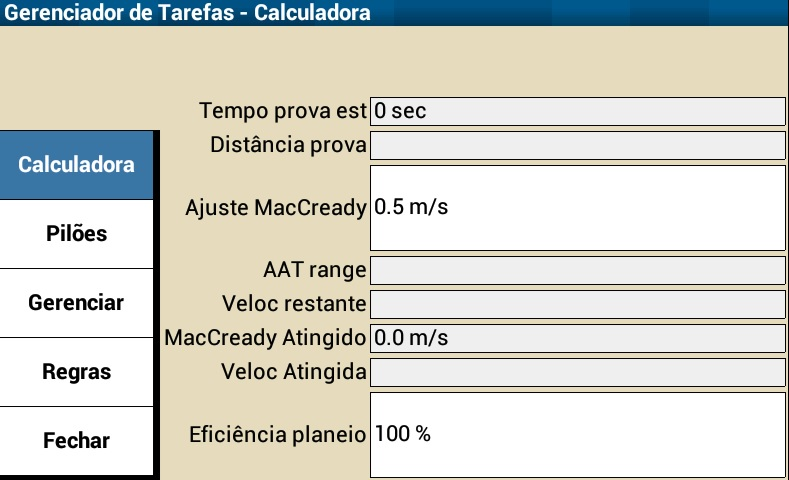
\includegraphics[angle=0,width=0.8\linewidth,keepaspectratio='true']{figures/dialog-taskcalculator.png}
\end{center}

\begin{description}
%\item[Tempo da prova]  Este campo mostra o tempo da prova.
\item[Tempo Prova est]  este campo mostra o tempo total para completar a prova usando o ajuste de MacCready introduzido.
\item[Task distance]  This field displays the task distance remaining.
\item[Ajuste MacCready]  permite ao usuário ajustar o MacCready e ver seus efeitos no tempo de prova estimado.
\item[AAT range]  permite ao usuário ajustar os alvos dentro das áreas AAT, para ver o efeito no tempo estimado e distância da prova.
\item[Velocidade restante]  este campo mostra a velocidade estimada restante para a prova com o ajuste MacCready fornecido.
\item[MacCready Atingido]  este campo mostra o valor de MacCready atingido.
\item[Veloc Atingida] mostra a velocidade atingida.
 % at the achieved MacCready setting???
\item[Eficiência planeio]  100\% indica um desempenho perfeito de MacCready, maior que 100\% indica que o desempenho de MacCready é superado voando em estradas de nuvens.  Menor que 100\% é apropriado se você voa consideravelmente fora da rota.  Este valor estima sua eficiência de cruzeiro de acordo com o histórico atual de vôo com o valor de MacCready.    Os cálculos iniciam após a prova iniciada.
\end{description}
Veja seção ~\ref{sec:task-speed-estim} para mais detalhes da velocidade da prova e cálculos de MacCready realizados.

Fechando a janela, o valor digitado de MacCready será usado como ajuste. Se o botão \bmenuw{Fechar} for pressionado, o ajuste de MacCready não será afetado.

O botão \bmenuw{Pilões} para provas AAT , ajusta o alcance (aumenta ou diminui) para que o tempo estimado exceda o tempo designado para prova subtraído de 5 minutos. O alcance é ajustado amplamente, geralmente todos os alvos são configurados para ''auto", significando que o piloto não tem que ajustar manualmente o alcance para achar o caminho para a chegada no tempo designado, diminuindo o trabalho do piloto.
  
\subsection*{Pilões}
Esta opção mostra uma lista ordenada de pontos da prova atual.
\menulabelr{\bmenuw{Pilões}} 
Se não houver waypoints na prova atual, só haverá a opção \bmenuw{Adicionar Pilão}.  Clicando no waypoint da lista e depois em \bmenug{Selec} o mesmo será incluso na lista.  

\subsection*{Gerenciar}
Esta página permite acionar todas as operações necessárias para criar novas provas ou gerenciar
\menulabelr{\bmenuw{Gerenciar}}as existentes.


\begin{itemize}
\item [\bmenuw{Nova Prova}] Apaga a prova atual e limpa as regras da prova, deixando os valores padrões.
\item [\bmenuw{Declarar}] Se houver um registrador externo conectado, permitirá que se envie a prova atual para o logger e faça a declaração.
\item [\bmenuw{Procurar}] Mostra uma lista de provas salvas, permitindo o piloto carregar uma prova já realizada.  Observe que esta opção irá sobrescrever a prova atual.
\item [\bmenuw{Salvar}] Salva a prova atual.  Clicando em 
  \bmenuw{Salvar} o piloto será questionado a entrar com um nome de arquivo para ser salvo.
\end{itemize}

\subsection*{Regras}
Os valores neste menu dependem do tipo de prova selecionado.  Clicando 
\menulabelr{\bmenuw{Regras}} em qualquer valor existente abrirá outro menu permitindo ao piloto selecionar um valor diferente para esta regra.  Os tipos de provas serão apresentados mais a frente.

Também clicando em \bmenuw{Regras} novamente, permite alternar entre uma visão geral da prova e retornar para a tela anterior.  

\section{Tipos de provas}
O XCSoar define três tipos diferentes de prova: Racing, AAT, e Insígnias/recordes FAI.

A descrição detalhada dos tipos de prova está listada adiante, mas este manual não pretende reformular as regras da FAI ou contestar os tipos de provas.  O leitor é forçado a se tornar familiar com cada tipo de prova, consultando as regras da FAI em \url{http://www.fai.org}. 


\subsection*{Competindo}
(Também conhecida como “prova atribuída”).  A prova atribuída envolve voar sobre alguns pilões em uma ordem específica.  Selecionando o tipo de prova permite ao piloto entrar com os seguintes parâmetros: 
  \begin{description}
  \item [Arm start manually] se ajustado para “Ligado”, alguns botões extras serão mostrados em ordem para \bmenug{Armar largada} bem como \bmenug{Desarmar largada} no menu \bmenug{Nav 1/2}, controlando a condição de detecção do Start.
  \item [Start open time] É a hora quando o Start deve abrir. 
  \item [Start close time] Hora em que a área de Start deverá fechar.
  \item [Veloc máx largada] esta é a velocidade máxima permitida na área de start.  Deve ter valor 0 se não houver limite.
  \item [Altura máx largada] maior altitude acima da altura de referência do start (AGL ou MSL), cuja prova pode ser iniciada.  Se não houver limites, o valor deverá ser 0.
  \item [Ref altura largada] especifica a altura máxima acima da altura de referência ao nível do solo do ponto de start (AGL ou MSL).
  \item [Altura mín chegada] Taltura mínima baseada na altura final de referência (AGL ou MSL) que a prova pode ser finalizada.  Deve ser ajustada em zero se não houver limite. 
  \item [Altura final de ref.] altura mínima referenciada ao nível do solo para o ponto final da prova (AGL ou MSL).
% \item [FAI start/finish rules] If enabled, this task type has no max. start height 
%   or max. start speed.  Finish height reference is set to AGL and finish height 
%   is 1000m below the start height \todonum[inline]{Is this description correct?}
  \end{description}
  
\subsection*{Área de prova atribuída (AAT) e Prova com área modificada (MAT)}
(Também conhecida como “prova de pilão” ou TAT).  Este tipo de prova é através de áreas designadas (restringidas às áreas com cilindros ou setores).  Há um tempo mínimo aplicado.  As opções de regras para esta prova incluem:
  \begin{description}
  \item [AAT min. time]  este é o tempo mínimo para realizar a prova. Consulte um especialista para as penalidades se finalizar em tempo abaixo do mínimo.  O tempo nesta opção é dado em minutos.
  \item [Outras regras] todas as outras regras permanecem as mesmas para este tipo de competição.
  \end{description}


\subsection*{Insígnias FAI / recordes}
  \begin{description}
  \item [Regras de início/ final FAI] se ajustado para “Ligado”, somente a hora de início pode ser definida.  Se a opção for “Desligado”, todas as outras regras da prova podem ser alteradas dos padrões da FAI.
  \end{description}

Uma vez definido o tipo de prova e as regras de início e fim também foram definidas conforme descrito acima, é necessário definir as propriedades de cada waypoint da prova.

\section{Regras da prova para os pilões}\label{sec:task-rules}

A janela de \bmenuw{Pilões} mostra uma lista de waypoint da prova. 
\menulabelr{\bmenuw{Pilões}} Se não houver pilões definidos, a tela irá mostrar uma lista vazia.  Com \bmenuw{Adicionar Pilão}, botões acima e abaixo, e \bmenug{Fazer Final} a lista é criada.  Os waypoints podem ser o ponto de início, pilão ou ponto final.  Selecione qualquer waypoint na lista ou clicando em \bmenug{Editar Ponto} mostrará as definições deste waypoint.  Clicando em \bmenuw{Mudar Tipo} mostrará uma série de opções de tipos de pilões disponíveis.  As definições de cada tipo são mostradas na parte inferior da tela.

Uma série de regras de prova podem ser usadas quando se monta uma prova, incluindo o triangulo FAI e Prova de Área Atribuída (AAT).  Muitas características da prova também podem ser personalizadas.

As linhas de início e fim são centralizadas nos seus waypoint e alinhadas perpendicularmente aos waypoints anteriores e posteriores, respectivamente.

Os pilões de setor são segmentos alinhados a 90° com a bissecção dos waypoints anteriores e posteriores, comumente usados em provas FAI.  Também há opções para os triângulos ingleses BGA e alemães DAeC.  

\subsection*{Tipos de start point}
As condições para se fazer o start dependem do tipo de início:
\begin{description}
\item[Start Cylinder] Quando a aeronave deixa a área do cilindro.
\item[Start Line] Quando a aeronave cruza a linha de início.
\end{description}

\subsection*{Tipos de pilões}
As condições para se fazer um pilão válido dependente de seu tipo:
\begin{description}
\item[Setor FAI] quando a aeronave entra na zona de observação (ZO), definida por um segmento e distância radial do waypoint.  O segmento é definido por um arco de 90° centrado sobre a bissetriz das pernas de entrada e saída, com distância de 20km.  
\item[Keyhole Sector (DAeC 0.5/10 sector)] é quando a aeronave entra em uma zona de observação, definida por um segmento e distância do waypoint. O segmento é definido por um arco de 90° centrado na bissetriz das pernas de entrada e saída, com distância de 10km.  A zona de observação também inclui um cilindro de 500m.
\item[Turnpoint Cylinder]  quando a aeronave entra em uma zona de observação definida por uma distância radial do waypoint.
\item[BGA Enhanced Option Fixed Course Sector]  quando a aeronave entra na zona de observação definida por um segmento e uma distância radial do waypoint.  O segmento é definido por um arco de 180° centrado na bissetriz das pernas de entrada e saída, com distância de 10km.  A zona de observação também inclui um cilindro de 500m (regras britânicas).
\item[Area Cylinder (AAT)]  e
\item[Area Sector (AAT)]  quando a aeronave entra na zona de observação definida por uma distância radial do waypoint e segmento para áreas de setores.

\end{description}

\subsection*{Tipos de Pontos Finais}
A realização da prova depende do tipo de ponto final.
\begin{description}
\item[Finish Cylinder] Quando a aeronave entra na área do cilindro.
\item[Finish Line] Quando a aeronave cruza a linha de chegada.
\end{description}

O avanço automático é disparado sempre que uma condição é alcançada.  Para iniciar uma prova AAT, mista ou Corrida, a prova tem que ser armada antes.

\tip As regras da competição podem ser definidas em um arquivo para serem distribuídas ao grupo de pilotos e comissão técnica, para que todos os competidores tenham as mesmas regras!

As regras adicionais da prova para inícios e finais válidos também devem ser especificadas.  O Start deve ter uma altitude máxima acima do solo e velocidade máxima definidas.  Os finais devem ter uma definição da altitude mínima acima do solo.  Estes parâmetros são definidos na página “Padrão das Provas”, nos ajustes das configurações.

Para provas não AAT, há opção disponível para ajustar a altura mínima final de acordo com a regra FAI, pela qual estabelece a altura mínima de chegada deve ser 1.000 metros acima da altura de largada.


%Need to add a section describing how to start the task%


\section{Avançando e reiniciando provas}\label{sec:advanc-rest-tasks}
Um waypoint, a qualquer tempo, pode ser atribuído como waypoint ativo na prova.  O waypoint ativo é usado para cálculos e mostrar informações de navegação, isto é, o piloto é direcionado a voar para este waypoint ativo (também conhecido como próximo waypoint na descrição do Infobox no Capítulo ~\ref{cha:infobox}).

Durante o vôo, a indicação de direção para o próximo waypoint é contínua.

A altitude necessária para completar a prova é calculada pela rota atual, iniciando com a posição atual da aeronave, passando pelos pilões até o ponto final.

A mudança do waypoint é feita automaticamente ou talvez manualmente.  O start da prova e pontos AAT são casos especiais que necessitam que se “arme” os pontos da prova antes que o sistema avançe para o próximo ponto da prova, uma vez que este ponto foi atingido.  Todos os pontos da prova serão avançados automaticamente ao próximo ponto assim que o último ponto for atingido.

Para provas não-Corrida, não é necessária nenhuma interação do usuário para avançar pela prova – o sistema irá automaticamente avançar a cada ponto da prova assim que o ponto for alcançado.  O piloto deve avançar ou retroceder manualmente o ponto ativo selecionando os menus, respectivamente:
 \bmenug{Nav}\blink\bmenug{Pto virada anterior} and
\bmenug{Nav}\blink\bmenug{Próx. Pto Virada}.

Os botões \bmenug{Pto virada anterior} e
\bmenug{Próx. Pto. Virada} mostram rótulos dinâmicos que indicam a ação a ser feita se selecionados.

Para os pontos de provas que necessitam serem armados, \bmenug{Próx. Pto. Virada} se torna 
\bmenug{Armar ponto} se o ponto não for armado;  se estiver armado, então aparecerá
\bmenug{Próx. Pto. Virada} permitindo o avanço manual.  O
\bmenug{Pto. virada anterior} aparecerá como\bmenug{Desarmar ponto}se o ponto estiver armado e vice versa.  Igualmente para provas de corrida, estes itens de menu se atualizam para armar os pontos de início.  Se o próximo ponto de virada é o ponto final, o rótulo se altera para tal.

As mensagens de estado são fornecidas para os pontos da prova que necessitam serem armados, como um lembrete para armar o ponto de virada quando o piloto está pronto para avançar ao próximo waypoint.  Para iniciar, é dado um alerta que a aeronave está no cilindro de start ou atrás da linha, como um lembrete de “armar” se necessário.  

Para PC e Pocket PC com tela de toque, o usuário pode manualmente navegar através dos waypoint selecionando a infobox do waypoint e apertando as setas para cima e para baixo.

Veja a seção ~\ref{sec:task-rules} para detalhes das regras de observação.

Se um usuário navegou até o waypoint manualmente, não significa que a aeronave passou efetivamente pelo waypoint!  Todavia, esta facilidade é útil para forçar um reinicio da prova ou para pular um waypoint quando se voa cross-country casual.

\tip As provas podem ser reiniciadas manualmente navegando através dos waypoint do início.

Em todos os modos, se a aeronave reentrar na zona de start ou cruzar o início do start anterior, a prova será automaticamente reiniciada.

Quando se seleciona  \bmenug{Pto. virada anterior}, o gatilho que detecta o auto avanço para aquele waypoint é apagado, significando que o gerenciador de prova aguarda a aeronave voar para aquela zona de observação (ZO) novamente antes de continuar a prova o piloto deve selecionar \bmenug{Próx. Pto. Virada} para avançar para o próximo waypoint da prova.

Um bip do sistema e uma mensagem é mostrada no avanço da prova/waypoint.  A mensagem é mostrada quando o sistema avança até o waypoint da prova automaticamente ou manualmente em modo “armado”, quando está armado e a aeronave está no setor:
\begin{description}
\item[Início da Prova]  aparece quando a aeronave cruzou o start ou saiu do setor de início.  Pode ser repetido a qualquer hora.
\item[Próx. Pto. Virada]  aparece quando a aeronave entrou no setor de observação para fazer o pilão.  Assim que o botão 
 \button{Armar virada} Para o modo de rearme manual, se a aeronave entrou no setor de observação, ao apertão este botão irá fazer o gerenciador de provas entender que a virada foi postergada para outro momento.
\item[Final da Prova]  aparece quando a aeronave cruzou a linha de chegada ou entrou no cilindro de final.  Ambos ocorrem no modo avançado. 
\end{description}


\section{Starts alternativos}\label{sec:alternate-starts}

%Alternate start points are skipped for XCsoar 6.0, but
%will potentially brought back in a next release. 

%\todonum[inline]{Alternate start points are skipped for XCsoar 6.0, but
%will potentially brought back in a next release. This section can thus be
%treated as obsolete. }

O sistema de provas permite que se defina start alternativos:

\blink\bmenuw{Pilões} selecione o início, \menulabelr{\bmenug{Nav 1/2}\blink
\bmenug{Prova}}\bmenuw{Editar Ponto}\blink\bmenuw{Habilitar Starts Alternados}

Na página de ponto de start do Gerenciador de Tarefas, mude para \bmenuw{Habilitar Starts Alternados}. Outra tela aparecerá para definir o ponto alternativo.  Neste caso, os pontos de start devem ter sidos definidos previamente.  Depois de selecionado \bmenuw{Habilitar Starts Alternados} e teclado \bmenuw{Edit Alternates}. Depois de selecionado\bmenuw{Add Alternates Starts} e pressionando 
\bmenuw{Realocar} abrirá a janela para seleção de waypoints.
 
Tendo configurado alguns starts alternativos, o método “próximo waypoint” será novamente aumentado.  Antes da detecção de um start válido e tendo armado o start manualmente, no menu de botões irá aparecer  \bmenug{Próximo Start}.

Resumindo, todos os rótulos dinâmicos em \bmenug{Nav 1/2} mostrarão os comandos a serem executados para selecionar os waypoints e condições, tanto na ordem normal como inversa.

%\begin{center}
%\includegraphics[angle=0,width=0.8\linewidth,keepaspectratio='true']{figures/%dialog-startpoint2.png}
%\end{center}
  
%  To edit the start points, move the cursor to an item in the list on
%  the right side of the dialogue, and press enter.  This opens the
%  waypoint selector dialogue, to allow selection of the waypoint.  This
%  process can be repeated several times for several alternate start
%  waypoints.  Press the `clear' button to clear all alternate start
%  points.

%  Each start sector is fixed to the same type (line/cylinder) and size
%  (start radius) defined in the task waypoint page.

%  Note that the task start point should be included in the alternate
%  start location list. 

%\begin{center}
%\includegraphics[angle=0,width=0.8\linewidth,keepaspectratio='true']{figures/%dialog-startpoint3.png}
%\end{center}

%\begin{center}
%\includegraphics[angle=0,width=0.8\linewidth,keepaspectratio='true']{figures/%dialog-startpoint4.png}
%\end{center}

%  In flight, any time you cross a start line (or exit a start
%  cylinder), this will start the task at that particular alternate
%  start.  Task statistics are recalculated for the start sector you
%  last flew through.  All alternate start sectors are shown on the
%  map.  You can re-start simply by flying through the start sector
%  again or another start sector.  This automatic re-start will only
%  happen if the active waypoint is the first turnpoint after the
%  start, or the start itself.

%  When the waypoint advance mode is `Arm' or `Arm Start', then a start
%  is only recognised by XCSoar if the advance trigger is armed.

%  If desired, alternate start points may be selected as the active
%  waypoint by selecting the previous waypoint.  Continuing to select
%  the previous waypoint will cycle through all alternate start points.

\section{Abortar/retomar a prova a Alternativos}

Se as condições atmosféricas ficarem piores, você poderá concluir que será impossível completar a prova.  Neste caso, você poderá instruir o XCSoar para “abortar” a prova e lhe orientar a procurar um pouso seguro.  Uma prova ordenada pode ser abortada de diversas maneiras, tanto pela seleção do waypoint e executar o comando ‘ir para’ ou acionando o modo de aborto.  Em ambos os casos, a prova atual poderá ser retomada.

\subsection*{Abortando a prova}\label{sec:taskabort}
Acionando o modo de aborto, força o XCSoar a entrar em modo especial de planeio final.  Para se aprofundar em modos de vôo, veja a seção \menulabelr{\bmenug{Nav 2/2}\blink\bmenug{Prova Abortar}}.  Para se aprofundar em modos de vôo, veja a seção  \ref{sec:flightmodes}. Neste modo de vôo, a opção de configuração “alcance polar” determina qual a altura de chegada do waypoint, usando o valor de segurança de MacCready para abortar a prova.  O padrão é usar o MacCready de segurança.  Quando se alterna para o modo de aborto, o valor de MacCready é alterado para seguro, mesmo que seja mais baixo que o valor atual em vôo.

Com o modo de aborto, a prova é desabilitada.  No mapa haverá pontos para os próximos pontos pousáveis para ajudar na decisão do piloto.  Enquanto durar o vôo, o grupo de pontos pousáveis é mantido permanentemente.  Os pontos pousáveis podem se alterar dinamicamente quando estiver em modo de aborto portanto, a qualquer momento vários pontos pousáveis são mostrados e qualquer um deles pode ser selecionado como waypoint ativo.  Mesmo que não haja ponto pousável dentro do planeio, os raios serão desenhados na tela
\sketch{figures/abort-low.png} 
Se as condições melhorarem, a prova pode ser retomada selecionando o mesmo botão de menu, agora indicando \bmenug{Prova Retomar}. O ponto ativo é então restaurado bem como todos os outros detalhes da prova.

\subsection*{Alternativos} \label{sec:alternates}
Os pontos alternativos são mantidos durante o vôo, refletindo que o piloto mantém seus olhos nestes pontos.\menulabelr{\bmenug{Nav 1/2}\blink
\bmenug{Alternativos}}.  Seis opções de pousos serão mantidas.  São filtradas pelos critérios de configuração (simples, prova ou casa). \config{alternatesmode} 
Escolhendo Prova ou Casa, há a inserção de alguns conceitos na apresentação dos alternativos, enquanto você está sendo orientado pela prova. 

Igualmente quando se tem toda a lista de waypoints, as informações adicionais podem ser vistas clicando em \bmenuw{Detalhes} antes de decidir para qual ponto se navegara.  Selecione um waypoint da lista e clique em \bmenuw{Ir Para}.
\sketch{figures/alternates_list.png}

Todavia, os itens na lista de alternativos obedecem regras diferentes e interagem da mesma forma com a prova atual.  Escolher um ponto na lista de alternativos aborta a prova; uma vez que as condições melhores, o resumo da prova pode ser realizado pelo botão já mencionado.


\section{Estado da prova }\label{sec:task-status}

A janela de diálogo de estado fornece um resumo das informações importantes da prova.   
\gesturespec{ldrdl} Pode ser útil para dar uma visão geral da prova enquanto se usa as Infoboxes por outros motivos.  A janela de estado pode ser consultada para se confirmar se um start válido foi detectad, bem como o progresso na prova
\menulabelr{\bmenug{Info 2}\blink\bmenug{Estado}}
.  Esta janela também pode ser acionada por menu ou gesto, descrevendo um “S”.   Pode-se ver as abas “Prova” e “Regras”.

A aba de prova mostra o tempo AAT, distâncias alcançadas, tempos restantes e da prova.  Aba das regras mostra a validação do start/final de acordo com as regras da prova.

\begin{center}
\begin{tabular}{c c}
Prova & Regras \\
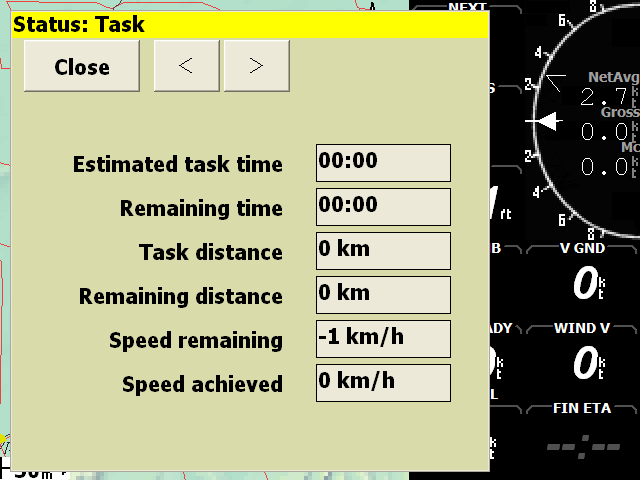
\includegraphics[angle=0,width=0.4\linewidth,keepaspectratio='true']{figures/status-task.png} &
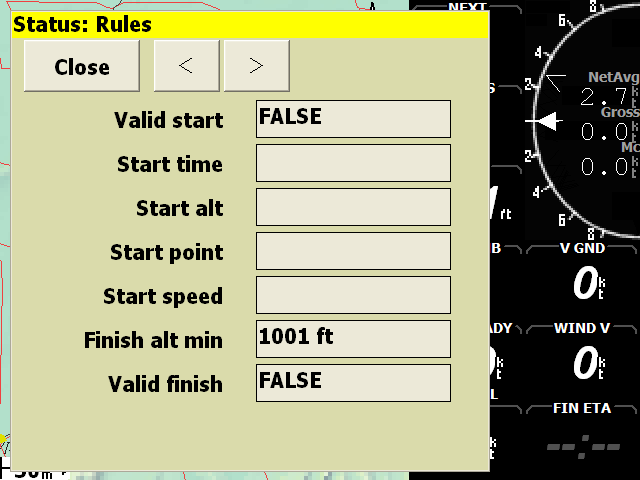
\includegraphics[angle=0,width=0.4\linewidth,keepaspectratio='true']{figures/status-rules.png} \\
\end{tabular}
\end{center}

\section{Provas de Áreas Atribuídas}\label{sec:aat-tasks}

\subsection*{Alvos AAT}

Um alvo é um ponto dentro de uma área AAT em que o piloto deve se dirigir.  Estes alvos podem ser movidos dentro da área AAT, portanto o piloto pode configurar a distância efetiva da prova.  Os alvos devem ser configurados no chão, durante o planejamento da prova e modificados durante o vôo.

Quando se voa uma prova AAT, o sistema de navegação direciona a aeronave para o alvo e as estatísticas como distância ao waypoint também são relativas ao alvo, ao invés do waypoint da área AAT.

O avanço automático do waypoint da prova não é acionado quando se entrar numa área AAT única.  O piloto tem que armar a virada manualmente para avançar para o próximo pilão.  Quando se arma um pilão AAT durante o vôo através da zona de observação, há o acionamento do modo de otimização da prova para capturar a realização dos alvos AAT e a atualização de toda a prova.   Veja a seção ~\ref{sec:advanc-rest-tasks} 
para mais detalhes.

\subsection*{Movendo manualmente os alvos}

Para fazer a especificação dos alvos diretamente, a localização destes é definida por alguns parâmetros que determinam quão longe da distância mínima ou máxima o alvo está. É expresso em porcentagem.  Por exemplo, um alcance ajustado em 100\%, o alvo é posicionado para fornecer a distância máxima possível de onde está o alvo.  Com o alcance ajustado em -100\%, o alvo é posicionado para fornecer a mínima distância total da prova.

O alcance zero determina a distância nominal da prova:  para setores, a prova é a metade da bissetriz radial; para cilindros, o alvo é o centro do cilindro.

A janela de cálculo de prova (veja seção ~\ref{sec:task-calc-dial}), mostra o percentual médio sobre todos os pilões do campo de alcance AAT.  Os alvos podem ser modificados individualmente através da janela de diálogo de cálculo de prova.


\subsection*{Alvos AAT e Calculadora de Prova}

O uso mais comum dos alvos quando se voa AAT são:
\begin{itemize}
\item Ajustar o MacCready esperado, lastro e ajustes de vento para o vôo, usando as janelas de configurações de vôo e ajustes de vento.
\item Definir a prova como normal através do editor de provas.
\item Baseado no julgamento do piloto de como está a condição e como algumas áreas são mais difíceis que outras, os alvos podem ser ajustados individualmente para cada pilão.  O campo ETE na visão do alvo comparado com o tempo mínimo assumido é mostrado como um Delta T para verificar se a prova planejada é eficiente e longa o suficiente.
\item Durante o vôo, se as situações mudarem como o ajuste de MacCready ou vento, a calculadora de prova pode ser mostrada para estimar o tempo de prova, novamente comparando com o tempo mínimo configurado para a prova.
\item Se o piloto decide estender ou reduzir o vôo, todos os pontos restantes podem ser modificados através da calculadora de prova.
\end{itemize}

A calculadora de prova também permite ao piloto perguntar (e ajudar na resposta) “O que acontece”, por exemplo: 
\begin{itemize}
\item O que acontece se as condições melhorarem? O ajuste de MacCready pode ser aumentado e o piloto pode ver se há ajustes suficientes para os alvos, bem como ser capaz de estender a prova.
\item O que acontece se as condições piorarem? O ajuste de MacCready pode ser diminuído e o piloto pode ver o quanto da prova pode ser reduzido a finalizar a prova mais tarde do que o tempo mínimo assumido.
\item O que acontecerá se eu deixar a área AAT agora?  Apertando  \button{Armar ponto} pode-se retirar a aeronave da posição atual e forçar uma otimização.  Os reposicionamentos dos pilões subsequentes podem ser revistos na janela calculadora de prova.
\end{itemize}

\subsection*{Projeção do alvo}

O XCSoar analisa continuamente o caminho que a aeronave percorre através de setores para localizar setores prévios AAT através do qual a distância de pontuação será a maior possível.  Internamente, o programa move os alvos para os setores prévios AAT, que podem ser os alvos otimizados.

Em algumas condições, os alvos do setor AAT atual podem ser movidos automaticamente:

\begin{itemize}
\item Quando dentro de um setor AAT, o alvo neste setor é movido para uma linha projetada deste o alvo do setor prévio até a aeronave, na mesma distância do alvo do setor prévio até a entrada do setor prévio.  Isto permite ao piloto escolher entrar em um setor AAT numa direção diferente ou compensar através da linha direta entre o alvo prévio e o atual.

\item Enquanto a aeronave estiver no setor AAT e a distância do alvo prévio até a aeronave for maior que a distância do alvo prévio até o alvo atual, o alvo é movido adiante, em cima da linha projetada com o alvo prévio até a aeronave, bem atrás da aeronave.  Conseqüentemente, a linha negra não será visível, mas uma seta azul otimizada que irá apontar na direção projetada.
\end{itemize}

São fornecidos exemplos nas próximas figuras para ilustrar como os alvos se movem durante um vôo e como o XCSoar determina o caminho de maior pontuação. 

\begin{maxipage}
\begin{center}
\begin{longtable}{|c|c|}
\toprule
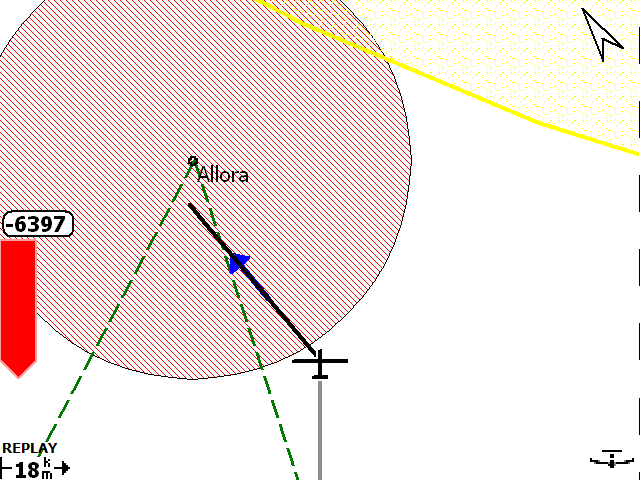
\includegraphics[angle=0,width=0.45\linewidth,keepaspectratio='true']{figures/faat01.png} & 
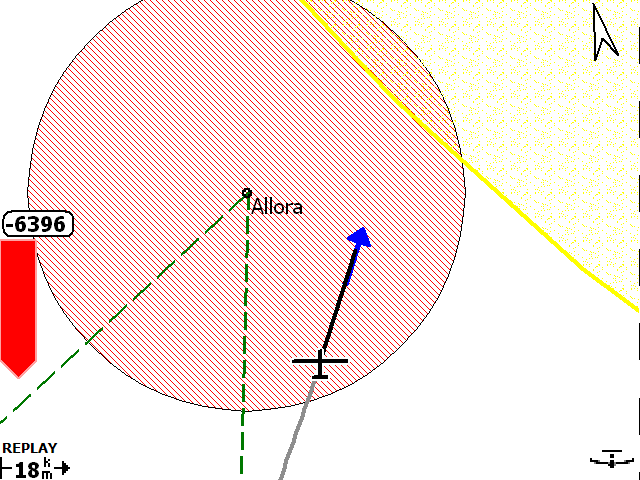
\includegraphics[angle=0,width=0.45\linewidth,keepaspectratio='true']{figures/faat02.png} \\
{\em Setor externo} & {\em Setor interno} \\
Alvo  (-20\%) está na bissetriz & Alvo  movido  ao longo da linha da trilha \\

\midrule
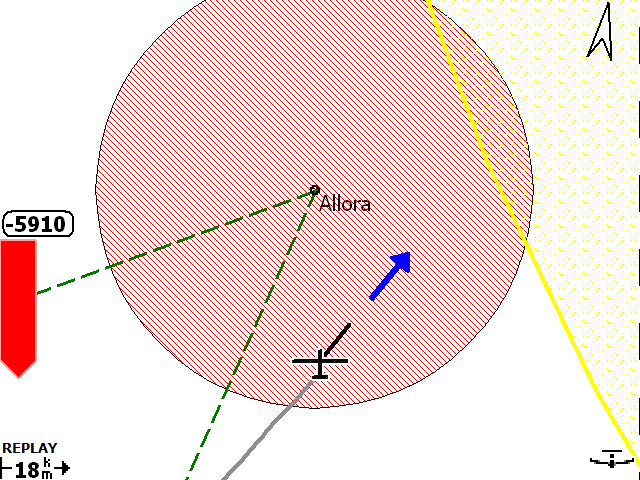
\includegraphics[angle=0,width=0.45\linewidth,keepaspectratio='true']{figures/faat03.png} & 
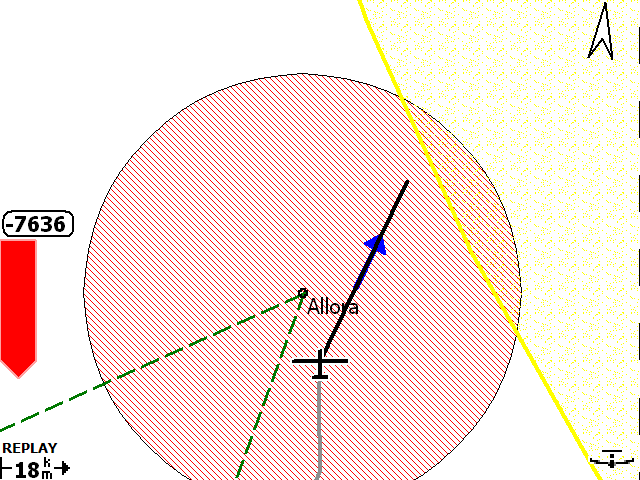
\includegraphics[angle=0,width=0.45\linewidth,keepaspectratio='true']{figures/faat04.png} \\
{\em Alcance diminuído pelo piloto} & {\em Alcance aumentado pelo piloto} \\
Alvo  (-80\%) movido ao longo da trilha & Alvo  (80\%) movido ao longo da trilha \\

\midrule
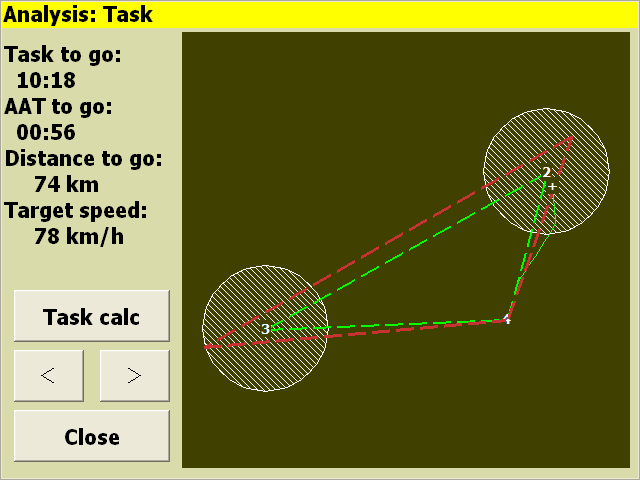
\includegraphics[angle=0,width=0.45\linewidth,keepaspectratio='true']{figures/faat05.png} & 
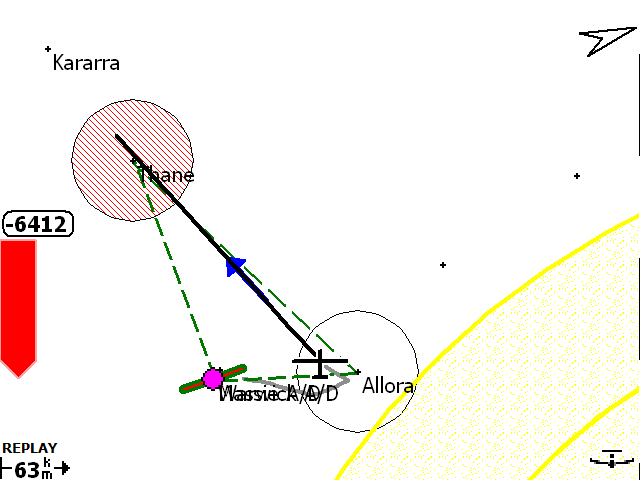
\includegraphics[angle=0,width=0.45\linewidth,keepaspectratio='true']{figures/faat06.png} \\
{\em Análise (página da prova)} & {\em Próximo waypoint} \\
Caminho em volta do alvo ativo  & “Armar Virada” acionado \\
\bottomrule
\end{longtable}
\end{center}
\end{maxipage}

\begin{maxipage}
\begin{center}
\begin{longtable}{|c|c|}
\toprule
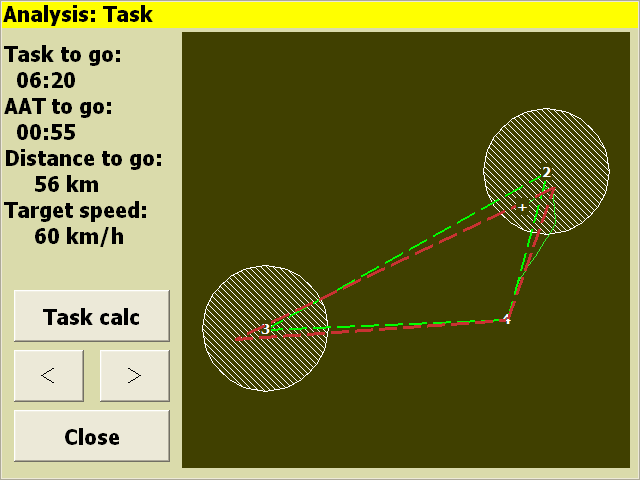
\includegraphics[angle=0,width=0.45\linewidth,keepaspectratio='true']{figures/faat07.png} & 
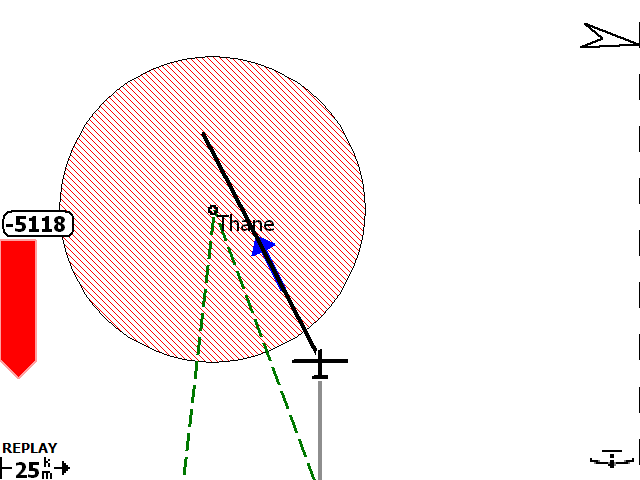
\includegraphics[angle=0,width=0.45\linewidth,keepaspectratio='true']{figures/faat08.png} \\
{\em Análise (página da prova)} & {\em Aproximando da próxima área} \\
Alvo de melhor pontuação encontrado & Alvo  (60\%) está na bissetriz \\

\midrule
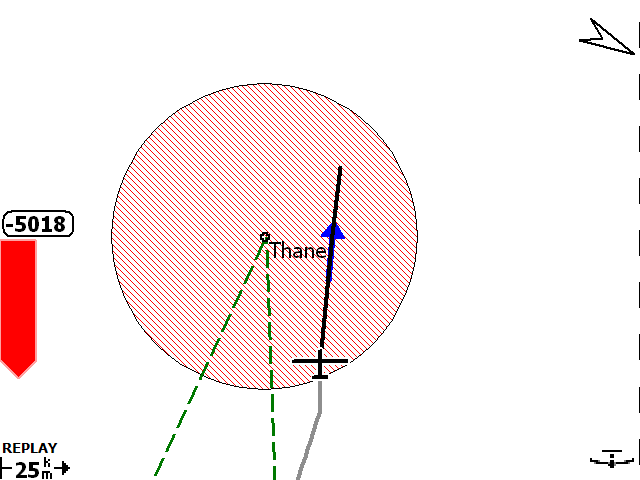
\includegraphics[angle=0,width=0.45\linewidth,keepaspectratio='true']{figures/faat09.png} & 
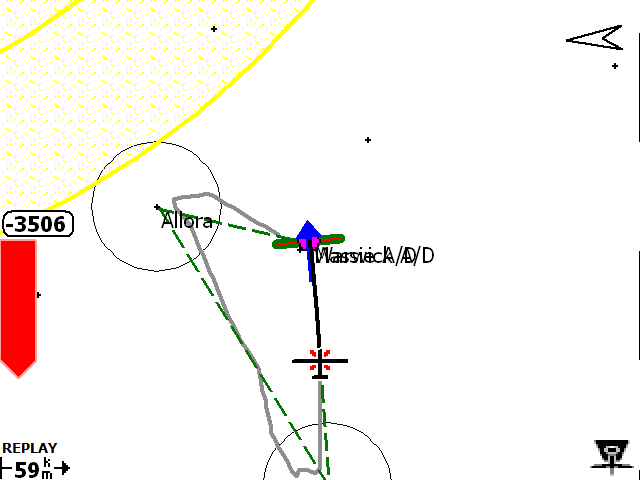
\includegraphics[angle=0,width=0.45\linewidth,keepaspectratio='true']{figures/faat11.png} \\
{\em Dentro do setor} & {\em Próximo waypoint} \\
Alvo  (60\%) movido ao longo da linha de trilha & Armar Virada Turn” pressionado \\

\midrule
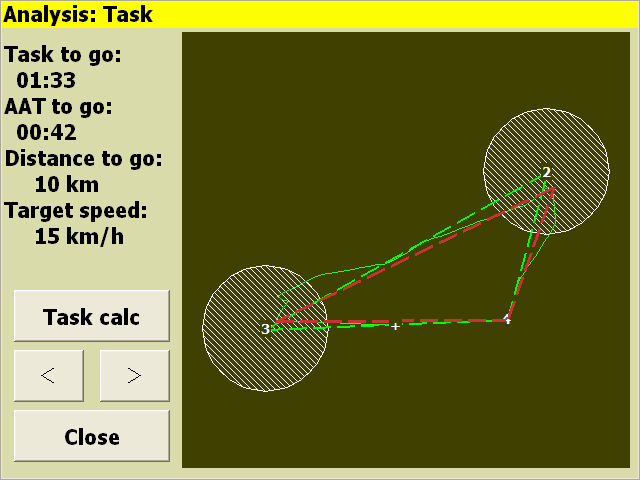
\includegraphics[angle=0,width=0.45\linewidth,keepaspectratio='true']{figures/faat12.png} &  \\
{\em Análise (página da prova)} &  \\
Alvo de melhor pontuação encontrado  &  \\

\bottomrule
\end{longtable}
\end{center}
\end{maxipage}

\section{Competição OnLine}

A janela de análise contém uma página chamada “Competição OnLine” pode ser usada para mostrar o caminho otimizado e estimar a pontuação. \config{taskrules} 
Os ajustes das configurações (página Gerenciador de Regras) permite que a seleção de quais conjuntos de regras podem ser usados para otimizar a distância OLC.

A otimização é feita continuamente em segundo plano e pode ser recuperada a qualquer momento.  A página de análise mostra uma visão geral gráfica do resultado da otimização, bem como distâncias e pontuação.  Há disponível um Infobox que fornece instantaneamente a distância OLC bem como a pontuação.

\begin{center}
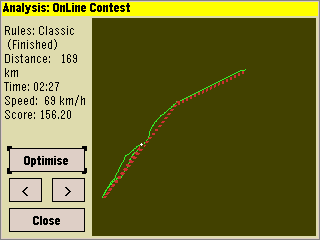
\includegraphics[angle=0,width=0.8\linewidth,keepaspectratio='true']{figures/shot-olc.png}
\end{center}

Quando se voa OLC, tanto nas provas AAT ou não-AAT, esta tela pode ser usada para gerenciar a navegação.  Durante o vôo, o computador irá otimizar o vôo atual respeitando as regras OLC selecionadas.

Na página de análise OLC, a trilha da aeronave é mostrada em uma linha fina verde e o caminho otimizado é mostrado como uma linha fina vermelha.

A pontuação e distância otimizada computada é aproximada.

Quando a aeronave pousar, os resultados mostrados não serão mais atualizados.



\section{Registrador}\label{sec:logger}

Pode ser usado um registrador de acordo com as especificações de arquivo IGC para gravar os voos.

Vários registradores de vôo são acessíveis através do XCSoar:

\begin{itemize}
\item Um registrador baseado em software.  Todas as versões do XCSoar têm esta funcionalidade.  O registrador é conforme padrões IGC mas não certificado. 
\item Por exemplo, a versão PRO do Altair tem um registrador interno certificado IGC.  O XCSoar comunica com registrador de dispositivos externos.
\item O XCSoar também pode enviar declarações aos registradores externos.  Para funcionar, o dispositivo tem que ser especificado nos ajustes das configurações.
 \config{comdevices} 
\item  Para alguns dos vários registradores, o XCSoar pode baixar arquivos IGC.  Isto é conveniente, especialmente para registradores que não são facilmente removíveis da aeronave.  
\end{itemize}

\subsection*{Configuração}
Uma tabela completa de características aceitas dos registradores está na seção~\ref{sec:supported-varios}.
A configuração é descrita em detalhes na seção ~\ref{conf:logger}.  Os detalhes dos arquivos ‘log’ estão na seção ~\ref{sec:logfiles}.

\subsection*{Ativação do Registrador}
O registrador pode ser ligado ou desligado automaticamente ou manualmente.  Para o Paraglider, o XCSoar fornece a opção de somente iniciar o registrador automaticamente. Assim, se estiver voando perto do terreno e muito devagar, o registrador não irá parar de registrar o vôo.  Se você escolher o início automático, o registrador irá parar somente no modo manual.  Para ligar ou desligar manualmente, selecione:
\sketch{figures/logger-startdeclare.png}
\begin{quote}
\bmenug{Config 3}\blink\bmenut{Registrador}{Iniciar}
\end{quote}

Quando o registrador interno do software estiver ativo, um pequeno led verde no canto inferior direito do mapa piscará por um segundo.

Por padrão, o XCSoar é ajustado para iniciar e parar automaticamente o registrador interno, quando detecta que a aeronave decolou e pousou, respectivamente.  Somente quando o registrador é iniciado manualmente é perguntado se deseja declarar a prova atual; quando é iniciado automaticamente já faz a declaração da prova atual.  No modo simulação, o registrador não é ativado automaticamente.

Se uma prova foi declarada e após houver a tentativa de modifica-la, haverá uma mensagem de alerta para confirmar que a ação tomada irá invalidar a declaração.  Isto é feito para dificultar a mudança acidentar da prova, resultando em falha na declaração da prova.

O software do registrador do XCSoar, quando iniciado, verifica por 500kb de espaço livre para salvar o arquivo.  Se não houver espaço, irá apagar os arquivos mais antigos para que libere espaço de até 500kb.  Não é exibida confirmação ao piloto quando esta ação é desempenhada. \warning

O software do registrador interno armazena dados até 60 segundos antes do seu início (automaticamente ou manualmente), ou seja, o início do vôo já foi gravado.  Isto significa que o software captura completamente a decolagem.

\subsection*{Replay do registrador}\label{sec:logger-replay}
Os registros de vôo no formato IGC gerados pelo XCSoar ou outros registradores podem ser vistos.  A janela Replay pode ser acessada através do menu:
\begin{quote}
\bmenug{Config 2}\blink\bmenug{Replay}
\end{quote}
\sketch{figures/loggerreplay.png}

Durante o replay, a palavra ‘REPLAY’ aparecerá no canto inferior esquerdo da tela.  O programa se comporta como se as atualizações reais do GPS estejam sendo recebidas.  A janela de Replay não precisa estar aberta durante o replay.

Para iniciar um replay do registo, primeiro selecione o arquivo para carregar e após 
\button{Iniciar}.  O replay pode ser feito em tempo acelerado mudando a escala de 1x até um número maior e pausado, se inserido valor zero.  Valores altos na escala podem degradar a estimativa de vento e outras rotinas de análise e estatísticas.

Pare o registrador usando   \button{Parar}.
Uma vez iniciado, apertando a tecla  \button{Iniciar} tem o feito de reiniciar o replay.

\tip É recomendado reiniciar o dispositivo antes de voar, depois que um arquivo de log foi visto, para se assegurar que as estatísticas internas do XCSoar foram devidamente zeradas.

Quando operar o XCSoar em modo FLY, o replay é desabilitado (parado) se o receptor de GPS detectar que a aeronave está se movendo.

O replay do registro trabalha melhor com altas taxas de amostragem de arquivos; um intervalo de 6 segundos ou menos é o ideal.


\subsection*{Erros analisando o registrador}\label{sec:raw-logger} Por uma simples razão de rastrear erros que o XCSoar pode conter, existe um registrador bruto.  No caso de você ser capaz de reproduzir um erro, você pode ativar o arquivo bruto de log por:
\begin{quote}
\bmenug{Config 3}\blink\bmenug{Raw Logger}
\end{quote}
Os desenvolvedores irão apreciar bastante a descrição de erros que inclua um arquivo de registro igual a este.  Facilita muito achar a causa raiz e analisá-la, economizando tempo para corrigir um erro.  

\section{Análise do vôos} \label{sec:analysis-climb}

A janela de análise é muito útil para se planejar e conduzir vôos de cross-country.  É acessada pelo menu: \gesture{Cima - Direita - Baixo}
\begin{quote}
\bmenug{Info 1}\blink\bmenug{Análise}
\end{quote}

Algumas páginas podem interessar:
\begin{description}
\item[Barógrafo]  mostra o histórico de altitude da aeronave.  As estatísticas são usadas para estimar a amplitude da térmica (base média e teto de subida) e para estimar como o teto está se alterando de acordo com o tempo.  As linhas da base e teto são desenhadas no barógrafo.

Os botões de ajustes abrem a janela de ajustes do vôo (ex. para ajustar o valor de QNH).  


\begin{center}
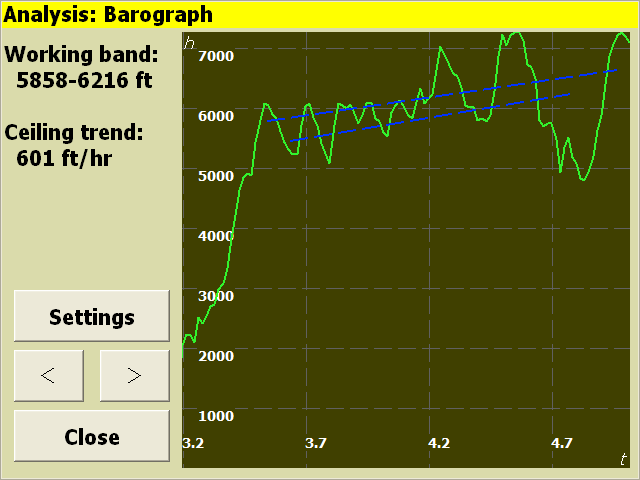
\includegraphics[angle=0,width=0.8\linewidth,keepaspectratio='true']{figures/analysis-barograph.png}
\end{center}

\item[Histórico de subida]
  :   mostra um gráfico com a taxa de subida média alcançada durante cada subida.  As estatísticas são utilizadas para estimar a taxa média de subida geral.  O valor atual de MacCready é mostrado no gráfico como uma linha pontilhada fina vermelha e a taxa de tendência é uma linha azul.

O botão “Calculadora” abre a calculadora de prova (ex. para ajustar o valor de MacCready).  


\begin{center}
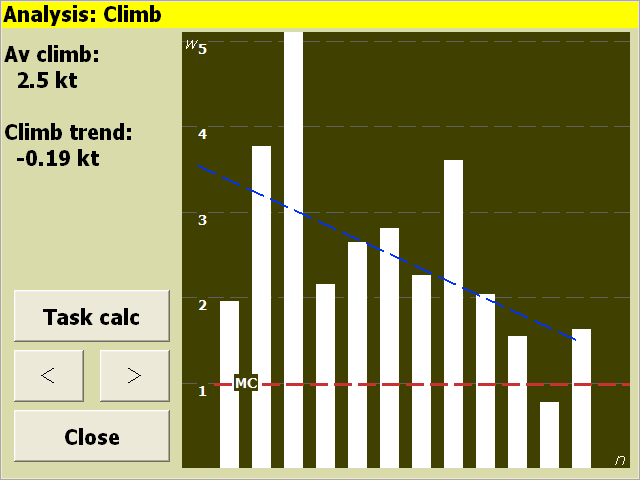
\includegraphics[angle=0,width=0.8\linewidth,keepaspectratio='true']{figures/analysis-climb.png}
\end{center}

\item[Prova]
 esta página mostra uma visão geral de toda a prova.  A prova principal é desenhada por uma linha pontilhada verde e as áreas AAT são sombreadas.  Para as provas AAT, o caminho da aeronave ao redor dos pilões restantes dentro das áreas AAT são mostrados em vermelho.  A trilha da aeronave é indicada por uma linha fina verde.

O botão “Calculador” abre a calculadora de prova (ex. para ajustar o alcance da prova AAT ou valor de MacCready).


\begin{center}
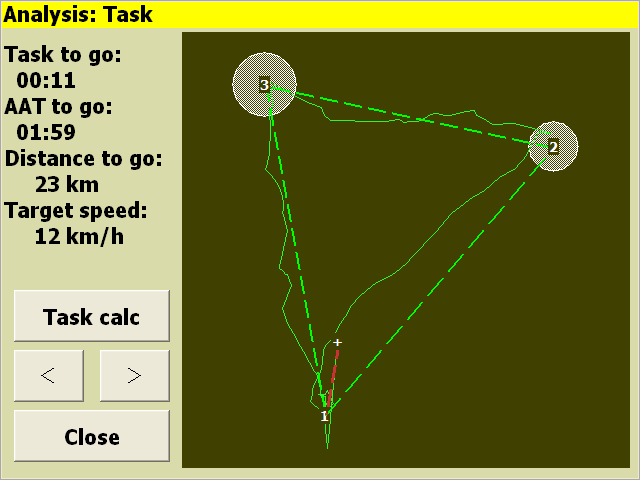
\includegraphics[angle=0,width=0.8\linewidth,keepaspectratio='true']{figures/analysis-task.png}
\end{center}

\end{description}

\section{Luz solar e hora}

O XCSoar computa a hora do nascer e pôr do sol, mostrado na janela de Estado da aeronave (veja seção ~\ref{sec:time-status}).  Observe que o terreno local e condições atmosféricas podem resultar em má visibilidade antes do pôr do sol.
Para sistemas PDA, o relógio é ajustado para a luz solar economizando tempo de acordo com os ajustes no menu de operação.  Para o Altair, o deslocamento de hora UTC deve ser ajustado manualmente para hora correta na janela de ajuste de configurações.
Se o tempo esperado de chegada no waypoint final da prova é posterior ao pôr do sol, haverá uma mensagem de alerta informando esta ação.

